\documentclass{article}
\usepackage[utf8]{inputenc}
\usepackage{amsmath,amssymb}
\usepackage{mathtools}
\usepackage{graphicx}
\usepackage{listings}
\usepackage[margin=1.2in]{geometry}

\usepackage{titling}
\usepackage{lipsum}

\usepackage{parskip}

\usepackage[
    style=authoryear-icomp,
    maxbibnames=9,
    maxcitenames=2,
    backend=biber
]{biblatex}
\addbibresource{sample.bib}

\setlength{\jot}{10pt}

\allowdisplaybreaks[1]

% Expectation symbol
\DeclareMathOperator*{\E}{\mathbb{E}}

% Math functions
\DeclareMathOperator{\Span}{span}

\graphicspath{{images/}}

\title{%
    Adversarial Text Generation\\
    \large NLP and Deep Learning --- Final Project
}

\author{%
    Andreas Holck Høeg-Petersen\\
    \texttt{anhh@itu.dk}
    \and
    Mathias Bastholm\\
    \texttt{mbas@itu.dk}
}

\begin{document}
\maketitle

\begin{abstract}
    \lipsum[1]
\end{abstract}

\section{Introduction}

In recent years, Generative Adversarial Networks (GANs) have gained a lot of
traction in the Deep Learning community because of their impressive results in
image generation. The general idea is that a generator and a discriminator are
jointly trained to produce an image output that is seemingly indistinguishable
from non-generated images. This model were first described
in~\cite{Goodfellow2014GenerativeAN}.

We want to attempt to apply this strategy for text generation. The main
difficulty for this task is that whereas image outputs can be considered a
continuous value, a sentence is inherently discrete as it is a sequence of words
each of which is chosen by the model using the non-differentiable $argmax$
function. To remedy this, we propose a model where the discriminator is trained
to distinguish between the continuous outputs of a pre-trained encoder given a
`true' sentence from the generated, `fake' output stemming from our generator.

\begin{figure}[h]
    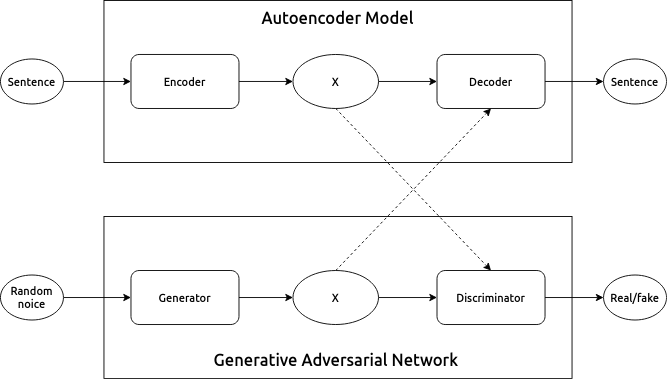
\includegraphics[width=\textwidth]{projectModel.png}
    \caption{% 
        Overview of the model architecture. The dotted lines from the
        $\mathbf{X}$s represents that the encoded and generated $\mathbf{X}$s
        will be fed to the discriminator and the decoder during training and
        evaluation, respectively.
    }\label{fig:projectModel}
\end{figure}

In our project, we will construct and train an autoencoder model that can encode
and decode a sentence from English to English. The encoded sentences are then
used as labelled training data for the discriminator, representing `true'
values. The job of the generator is to produce similar encodings but doing this
from random noise in a way that makes the discriminator unable to distinguish
between the encodings stemming from the autoencoder and the encodings stemming
from the generator.

Ideally, this would train the generator to produce sentence encodings that can
be fed to the decoder of the Transformer model which would then produce
meaningful sentences from this artificially generated input. See
Figure~\ref{fig:projectModel} for an overview of the complete model.

This project thus have two objectives: one is to construct a working autoencoder
that can map an English sentence to some hidden state $\mathbf{X}$ with a
corresponding decoder that can extract the original sentence from $\mathbf{X}$.
For convenience, we will refer to the encoder part of this model as the
`Teacher'. The second objective is to build a GAN network, where a generator ---
the `Student' --- must learn to produce approximations of $\mathbf{X}$.

The second objective is highly experimental as explained in
Section~\ref{sec:background}, where we will also describe other approaches at
using the GAN architecture for NLP problems. In Section~\ref{sec:method} we will
describe how we have build the different parts of the model and how we utilize
our dataset. Then in Section~\ref{sec:analysis} we will present our results and
discuss the shortcomings of the model\(s\), and in
Section~\ref{sec:furtherResearch} we will proceed to suggest improvements and
ideas for further research. Lastly, in Section~\ref{sec:conclusion} we conclude
on our project.


\section{Background}\label{sec:background}

\lipsum[4]

\section{Method}\label{sec:method}


\subsection{Baseline}


\subsection{Dataset}\label{sec:dataset}


\subsection{Models}\label{sec:models}


\subsection{Training}\label{sec:training}


\section{Analysis}\label{sec:analysis}


\subsection{Results}\label{sec:results}


\subsection{Discussion}\label{sec:discussion}


\section{Further research}\label{sec:furtherResearch}


\section{Conclusion}\label{sec:conclusion}


\printbibliography%

\end{document}

